To test the installation first go to the examples \lstinline{cd tutorial/examples/} and run the following Hello World like example \lstinline{python3 intro_basic.py} to test the installation. The first example shows a CPlantBox simulation. The main steps are how to open a CPlantBox parameter file (L13), perform the simulation (L20), save the results (L23-L26), and make an interactive plot showing the results (L29). Figure \ref{fig:intro_basic} shows the expected simulation result.  

\lstinputlisting[language=Python, caption=Basic example]{examples/intro_basic.py} 

\noindent 
Lets revise the above code in more detail: 
\begin{itemize}
 \item[2] We add the path to find the \emph{plantbox} module.
 \item[4] Imports the CPlantBox Python library \emph{plantbox} and name it pb.
 \item[5] Imports a auxiliary script for visualization of the rootsystem with VTK and name it vp.
 \item[8] Constructs the plant object.
 \item[12] Opens an .xml containing parameters describing the structural properties of the plant by defining the seed (SeedRandomParameters), the stem (StemRandomParameters), the leaf (LeafRandomParameters) and the roots (RootRandomParameters). Alternatively, all parameter can be set or modified directly in Python. A more detailed description is given in Section \ref{sec:cplantobx}.
 \item[16] Initializes the simulation: Creates the initial stem, tap root and the base roots
 (i.e. all basal roots, and shoot borne roots that might emerge). Initializes the tropisms and passing the domain geometry, 
 and creates the elongation functions. 
 \item[20] Performs the simulation. The value 40 is the simulation time in days. If no simulation time is passed the simulation time is taken from the parameter file. Note that simulation results are independent from the time step, i.e. 40 simulate(1) calls should yield a similar result 
 as simulate(40) (due to stochasticity we cannot expect the exact same result). 
 \item[23] Saves the resulting plant geometry in the VTK Polygonal Data format (VTP) where each plant organ is repesented as a polylines. Use Paraview to visualize the results, see Section \ref{ssec:visualisation}.
 \item[25,26] If we want to visualize simulation results that are given per segment another option is to export the plant geometry segment wise. L25 creates a segment based representation of the plant geometry, and L26 saves it as VTP file.
 \item[29] Create an interactive plot (use mouse to rotate or zoom) using VTK. Per default plant 'age', 'creationTime', 'radius','organType' or 'subType' can be viusalized. The organType is 1 for the seed, 2 for root, 3 for stem, and 4 for leafs. The subType is the number of the parameter set within a organ class, i.e. the type of root, stem or leaf. You can rotate (left click) pan (right click) or zoom (mouse wheel) and save a screenshot as png file by pressing 'g', or reset view 'r', or change view by pressing 'x', 'y', 'z', and 'v'.
 \end{itemize}
  
\begin{figure}
\centering
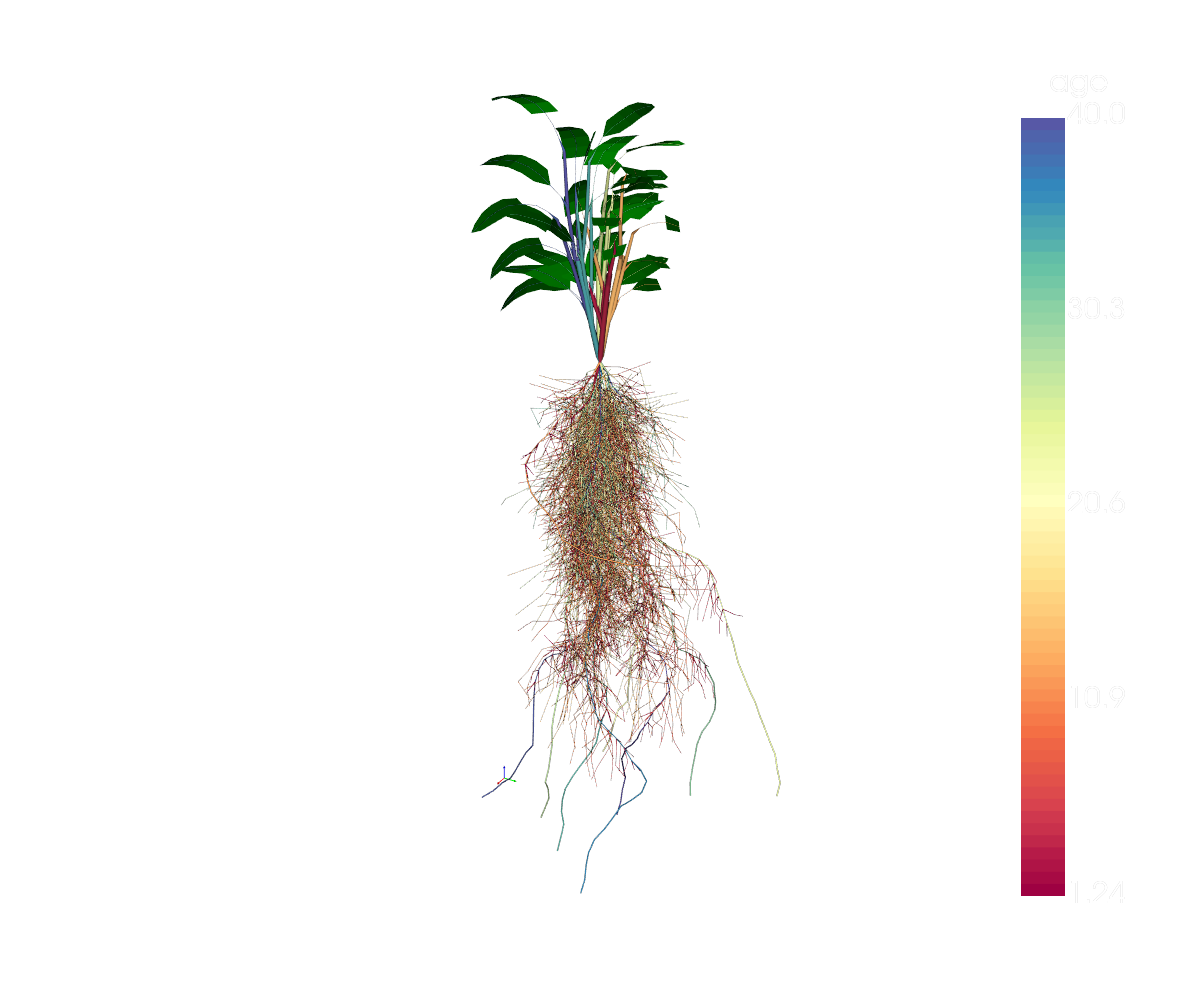
\includegraphics[width=0.5\textwidth]{examples/results/intro_basic.png} 
\caption{Plant after 40 days simulation time.} \label{fig:intro_basic}
\end{figure}  
